
\section{User Defined Forces}
\label{section:userdef}


%\subsection{Applied Forces and Analysis}

There are several ways to apply external forces to simulations with \NAMD.
These are described below.


\subsection{Constant Forces}

NAMD provides the ability to apply constant forces to some atoms.
There are three parameters that control this feature.

\begin{itemize}

\item
\NAMDCONFWDEF{constantForce}{Apply constant forces?}{yes or no}{no}
{Specifies whether or not constant forces are applied.}

\item
\NAMDCONF{consForceFile}{PDB file containing forces to be applied}{UNIX filename}
{
The X, Y, Z and occupancy (O) fields of this file are read to
determine the constant force vector of each atom, which is
(X,Y,Z)*O, in unit of kcal/(mol*\AA). The occupancy (O) serves as
a scaling factor, which could expand the range of the force
applied. (One may be unable to record very large or very small
numbers in the data fields of a PDB file due to limited space).
Zero forces are ignored.

Specifying {\tt consforcefile} is optional; constant forces may be specified
or updated between runs by using the \icommand{consForceConfig} command.
}

\item
\NAMDCONFWDEF{consForceScaling}{Scaling factor for constant forces}{decimal}{1.0}
{Scaling factor by which constant forces are multiplied.  May be changed between run commands.}

\end{itemize}


\subsection{External Electric Field}

\NAMD\ provides the ability to apply a constant electric field to the molecular
system being simulated.
Energy due to the external field will be reported in the MISC column
and will be continuous even in simulations using periodic boundary conditions
as unwrapped coordinates are used to calculate energy and pressure,
resulting in linearly increasing pressure over time for systems with free ions.
To avoid this effect, for periodic simulations the new {\tt eFieldNormalized} option
should be used with the electric field vector multiplied by the cell dimension.
There are three parameters that control this feature.

\begin{itemize}

\item
\NAMDCONFWDEF{eFieldOn}{apply electric field?}{{\tt yes} or {\tt no}}{{\tt no}}
{Specifies whether or not an electric field is applied.}

\item
\NAMDCONF{eField}{electric field vector}{vector of decimals (x y z)}
{Vector which describes the electric field to be applied.
Units are ${\rm kcal} / ({\rm mol \; \AA} \; e)$, which is natural for simulations.
This parameter may be changed between {\tt run} commands, allowing a square
wave or other approximate wave form to be applied.}

\item
\NAMDCONFWDEF{eFieldNormalized}{electric field vector scaled by cell basis vectors?}{{\tt yes} or {\tt no}}{{\tt no}}
{Specifies whether or not that eField vector has been scaled by the cell basis vectors,
thus indicating the voltage drop across the cell in units of ${\rm kcal} / ({\rm mol} \; e)$.
The eField vector is then scaled by the reciprocal lattice vectors at each timestep.
When eFieldNormalized is true the eField forces do not contribute to the pressure calculation.}

\end{itemize}

\subsection{Grid Forces}

\NAMD\ provides the ability to specify grids describing a potential in the simulation 
space. Each atom is affected by the potential based on its charge and its position, 
using the potential function interpolated from the specified grid(s). Energy due to the 
grid-defined field will be reported in the MISC column of the output, unless a scaling
factor not proportional to (1,1,1) is used.

NAMD allows the definition of multiple grids, each with a separate set of defining 
parameters. This is specified using a tag field in each of the mgridforceXXX commands. 
The tag is an alphanumeric string without spaces which identifies to which grid the 
specified field applies.

The grid file format is a subset of the DataExplorer DX file format, as shown below:
\begin{verbatim}
# Lines at the beginning of the file starting with a # symbol 
# are ignored as comments
# Variables (replaced by numbers in an actual file):
#   xn, yn, and zn are the number of data points along each dimension;
#   xorg, yorg, and zorg is the origin of the grid, in angstroms;
#   x[1-3]del, y[1-3]del, and z[1-3]del are the basis vectors which transform
#   grid indices to coordinates in angstroms:
#      x(i,j,k) = xorg + i * x1del + j * y1del + k * z1del
#      y(i,j,k) = yorg + i * x2del + j * y2del + k * z2del
#      z(i,j,k) = zorg + i * x3del + j * y3del + k * z3del
#
#   Grid data follows, with three values per line, ordered z fast, y medium,
#   and x slow. Exactly xn*yn*zn values should be given. Grid data is then
#   terminated with a field object.
#   
#  Note: Other features of the DX file format are not handled by this code
#
object 1 class gridpositions counts xn yn zn
origin xorg yorg zorg
delta x1del y1del z1del
delta x2del y2del z2del
delta x3del y3del z3del
object 2 class gridconnections counts xn yn zn
object 3 class array type double rank 0 items [ xn*yn*zn ] data follows
f1 f2 f3
f4 f5 f6
.
.
.
object 4 class field
component "positions" value 1
component "connections" value 2
component "data" value 3
\end{verbatim}

Each dimension of the grid may be specified as continuous or not. If the grid is not continuous in a particular dimension, the potential grid is padded with one border slices on each non-continuous face of the grid, and border grid values are computed so that the force felt by an atom outside the grid goes to zero. If the grid is continuous along a particular dimension, atoms outside the grid are affected by a potential that is interpolated from the grid and its corresponding periodic image along that dimension.

To calculate the force on an atom due to the grid, the atom's coordinates are transformed according to the current basis vectors of the simulation box to a coordinate frame that is centered at the center of the specified grid. Note that the size and spatial coordinates of the grid remain fixed, and are not scaled as the size of the simulation box fluctuates. For atoms within the grid, the force is computed by analytically determining the gradient of the tricubic polynomial used to interpolate the potential from surrounding grid values. For atoms outside the grid, the state of the {\tt mgridforcecont[1,2,3]} determine whether the force is zero, or computed from the images of the grid as described above. Note that if the grid is ever larger than the periodic box, it is truncated at the edge of that box. The consequence of this is that the computed potential will not vary smoothly at the edges, introducing numerical instability.

NAMD also supports non-uniform grids, allowing regions of a grid to be defined at higher resolution.
Non-uniform grids are structured hierarchically, with a single \emph{maingrid} which has one or more \emph{subgrid}s.
Each subgrid spans a number of maingrid cells in each of the three dimensions, and effectively redefines the data in that region.
The subgrids are usually defined at higher resolution, with the restriction that the number of cells along each dimension is an integral number of the original number in the maingrid.
Note that the maingrid still has data points in regions where subgrids are defined, and that, on the boundary of a subgrid, \emph{they must agree with the values in the subgrid}.
Subgrids, in turn, may have subgrids of their own, which may have subgrids of their own, etc.

A non-uniform grid file takes the form of a special comment block followed by multiple normal grid definitions.
The special comment block defines the grid hierarchy, and consists of comments beginning with {\tt \# namdnugrid}.
An example follows:
\begin{verbatim}
# namdnugrid version 1.0
# namdnugrid maingrid subgrids count 2
# namdnugrid subgrid 1 generation 1 min x1 y1 z1 max x2 y2 z2 subgrids count 2
# namdnugrid subgrid 2 generation 2 min x3 y3 z3 max x4 y4 z4 subgrids count 0
# namdnugrid subgrid 3 generation 2 min x5 y5 z5 max x6 y6 z6 subgrids count 0
# namdnugrid subgrid 4 generation 1 min x7 y7 z7 max x8 y8 z8 subgrids count 0
\end{verbatim}
The maingrid is described by the number of subgrids.
Subgrids are additionally described by a subgrid number; a generation number, which should be one higher than the generation of its supergrid; and {\tt min} and {\tt max} attributes, which describe the location of the subgrid within its supergrid.
In this example, the maingrid has two subgrids, subgrid 1 and subgrid 4, labeled {\tt generation 1}.
The first of these subgrids has two subgrids of its own ({\tt generation 2}).
Notice that subgrids are described immediately after their supergrid.
The {\tt min} and {\tt max} attributes are given in units of grid \emph{cells} of the supergrid.
For example, a subgrid with {\tt min 0 0 0 max 1 1 1} would redefine 8 cells of its supergrid, the space between gridpoints (0, 0, 0) and (2, 2, 2) in grid coordinates.
Following the comment block, the maingrid and subgrids are defined in the format described above, in the same order as the comment block.


The following parameters describe the grid-based potentials.

\begin{itemize}

\item
\NAMDCONFWDEF{mgridforce}
{apply grid forces?}
{{\tt yes} or {\tt no}}{{\tt no}}
{Specifies whether or not any grid forces are being applied.}

\item
\NAMDCONFTAG{mgridforcefile}
{PDB file specifying force multipliers and charges for each atomd}
{UNIX file name}
{The force on each atom is scaled by the corresponding value in this PDB file. By setting the force multiplier to zero for an atom, it will not be affected by the grid force. }

\item
\NAMDCONFTAGWDEF{mgridforcecol}
{column of PDB from which to read force multipliers}
{X, Y, Z, O, or B}
{B}
{Which column in the PDB file specified by {\tt mgridforcefile} contains the scaling factor}

\item
\NAMDCONFTAGWDEF{mgridforcechargecol}
{column of PDB from which to read atom charges}
{X, Y, Z, O, or B}
{Atom charge used for electrostatics.} 
{Which column in the PDB file specified by {\tt mgridforcefile} contains the atom charge. By default, the charge value specified for the short-range Columb interactions are also used for the grid force. Both {\tt mgridforcecol} and {\tt mgridforceqcol} can be specified, in which case the apparent charge of the atom will be the product of the two values.}

\item
\NAMDCONFTAG{mgridforcepotfile}
{grid potential file name}
{UNIX file name}
{File specifying the grid size, coordinates, and potential values.}

\item
\NAMDCONFTAGWDEF{mgridforcevolts}
{grid potential units in eV/charge}
{{\tt yes} or {\tt no}}{{\tt no}}
{If set, the grid potential values are expressed in {\rm eV}. Otherwise, values are
in ${\rm kcal} / ({\rm mol} \; charge)$}

\item
\NAMDCONFTAGWDEF{mgridforcescale}
{scale factor for grid potential}
{Vector of decimals {\it scale}$_x$ {\it scale}$_y$ {\it scale}$_z$ }
{1 1 1}
{Defines the scale factors that modulate the amplitude of the grid potential forces in each dimension.
  When the three values are the same number, the grid potential's value is also included in the MISC column of the energy output.
  After initialization, the three scale factors may be updated between ``run'' commands by the {\tt updategridforcescale} command.
  In the special case when ``0 0 0'' is given for this option, the corresponding grid potential can be used a collective variable in the Colvars module (Sec.~\ref{section:colvars}), allowing the use of restraint potentials and fully time-dependent forces.}

\item
\NAMDCONFTAGWDEF{updategridforcescale}
{scale factor for grid potential}
{Vector of decimals {\it scale}$_x$ {\it scale}$_y$ {\it scale}$_z$ }
{1 1 1}
{Provides new scale factors to be applied to the grid potential values. This comand can be issued between ``run'' commands to modify the amplitude of the grid potential. The values provided remain constant for the duration of each ``run'' command.}


\item
\NAMDCONFTAGWDEF{mgridforcecont1}
{Is grid continuous in the direction of the first basis vector}
{{\tt yes} or {\tt no}}{{\tt no}}
{By specifying that the grid is continuous in a direction, atoms outside of the grid will be affected by a force determined by interpolating based on the values at the edge of the grid with the values of the corresponding edge of the periodic image of the grid. The current size of the simulation box is taken into account, so that as the simulation box size fluctuates, the force on an atom outside of the grid varies continuously until it re-enters the opposite edge of the grid. If the grid is not continuous in this direction, the interpolated force on atoms near the edge of the grid is calculated so that it continuously approaches zero as an atom approaches the edge of the grid.}

\item
\NAMDCONFTAGWDEF{mgridforcecont2}
{Is grid continuous in the direction of the second basis vector}
{{\tt yes} or {\tt no}}{{\tt no}}
{Operates the same as {\tt mgridforcecont1} except applies in the direction of the second basis vector}

\item
\NAMDCONFTAGWDEF{mgridforcecont3}
{Is grid continuous in the direction of the third basis vector}
{{\tt yes} or {\tt no}}{{\tt no}}
{Operates the same as {\tt mgridforcecont1} except applies in the direction of the third basis vector}

\item
\NAMDCONFTAGWDEF{mgridforcevoff}
{Offset periodic images of the grid by specified amounts}
{vector of decimals (x y z)}
{(0 0 0)}
{If a continuous grid is used along a particular basis vector, it may be desirable to shift the potentials in the image to manipulate the potential outside the grid. For example, consider the case where the potential is a ramp in the $x$ direction and the grid is defined for points $[0,N)$, with a potential $f(i,j,k)$ given by $f(i,j,k) = f_0 + i (f_1-f_0) / N$. By shifting the images of the grid, the potential can be transformed as illustrated in Fig.~\ref{fig:gridshift}.
}

\begin{figure}[htb]
  \center{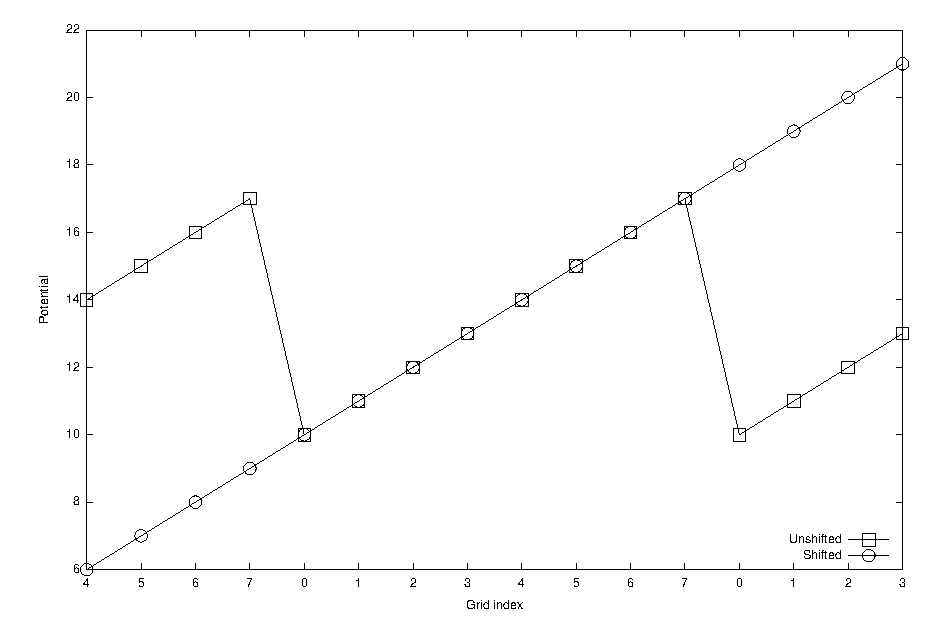
\includegraphics{figures/gridshift}}
  \caption[Graph showing a slice of a ramp potential, showing the effect of 
           {\tt mgridforcevoff}]
  {\small Graph showing a slice of a ramp potential, with eight grid points along the axis, and a periodic cell size which just contains the grid. The Unshifted case shows how the pontential is not smooth when {\tt mgridforcevoff} is not specified, or set to zero. The Shifted potential shows the grid that results when {\tt mgridfocevoff} is set so that the wrapped potential is offset so that the potential has constant slope at the periodic boundaries.}
  \label{fig:gridshift}
\end{figure}

\item
\NAMDCONFTAGWDEF{mgridforcelite}
{Is grid to use Gridforce Lite interpolation?}
{{\tt yes} or {\tt no}}
{{\tt no}}
{When Gridforce Lite is enabled, a faster but less accurate interpolation method is used to compute forces.
Specifically, rather than computing a tri-cubic interpolation of the potential, from which the force is then computed analytically, Gridforce Lite computes force as a linear interpolation.
This method also increases the memory required by Gridforce.
Note that Gridforce Lite is incompatible with use of the {\tt mgridforcecont[123]} keywords and with non-uniform grids.
}

\end{itemize}

\subsection{Moving Constraints}

Moving constraints feature works in conjunction with the Harmonic
Constraints (see an appropriate section of the User's guide).
The reference positions of all constraints
will move according to
\begin{equation}
\label{eq:smdrefpos}
   \vec r(t) \; = \; \vec r_0 \, + \, \vec v t \,.
\end{equation}
A velocity vector $\vec v$ ({\tt movingConsVel}) needs to be specified.

The way the moving constraints work is that the moving reference
position is calculated every integration time step using
Eq.~\ref{eq:smdrefpos}, where $\vec v$ is in \AA/timestep, and $t$ is the
current timestep (i.e., {\tt firstTimestep} plus however many
timesteps have passed since the beginning of \NAMD\ run). Therefore,
one should be careful when restarting simulations to appropriately
update the {\tt firstTimestep} parameter in the \NAMD\ configuration
file or the reference position specified in the reference PDB file.

\noindent {\bf NOTE: } \NAMD\ actually calculates the constraints
potential with $U = k (x-x_0)^d$ and the force with $F = d k (x-x_0)$,
where $d$ is the exponent {\tt consexp}. The result is that if one
specifies some value for the force constant $k$ in the PDB file,
effectively, the force constant is $2 k$ in calculations. This caveat
was removed in SMD feature.

The following parameters describe the parameters for the
moving harmonic constraint feature of \NAMD.

\begin{itemize}

\item
\NAMDCONFWDEF{movingConstraints}{Are moving constraints active}
{{\tt on} or {\tt off}}{{\tt off}}
{Should moving restraints be applied to the system. If set
to {\tt on}, then  {\tt movingConsVel} must be defined.
May not be used with {\tt rotConstraints}.}

\item
\NAMDCONF{movingConsVel}{Velocity of the reference position movement}
{vector in \AA/timestep}
{The velocity of the reference position movement. Gives both absolute
value and direction}

\end{itemize}

\subsection{Rotating Constraints}

The constraints parameters are specified in the same manner as for
usual (static) harmonic constraints. The reference positions of all
constrained atoms are then rotated with a given angular velocity
about a given axis. If the force constant of the constraints is
sufficiently
large, the constrained atoms will follow their reference positions.

A rotation matrix $M$ about the axis unit vector $v$ is calculated every
timestep
for the angle of rotation corresponding to the current timestep.
    angle = $\Omega t$,
where $\Omega$ is the angular velocity of rotation.

From now on, all quantities are 3D vectors, except the matrix $M$ and the
force constant $K$.

The current reference position $R$ is calculated from the initial
reference
position $R_0$ (at $t=0$),
    $R = M (R_0 - P) + P$,
where $P$ is the pivot point.

%geometry of rotation:
%
%
%
%                        * R
%                      / |
%                    /   |
%                  /     | normal to axis
%                /       |
%            P /         |
%        ----*--->-------*---------------------> axis
%                v       N

Coordinates of point N can be found as
   $N = P + ( (R - P) \cdot v ) v$.
Normal from the atom pos to the axis is, similarly,
   normal $= ( P + ( (X - P) \cdot v ) v ) - X$
The force is, as usual,
   $F = K (R - X)$;
This is the force applied to the atom in NAMD (see below).
NAMD does not know anything about the torque
applied. However, the torque applied to the atom can be calculated
as a vector product
   torque $= F \times normal$
Finally, the torque applied to the atom with respect to the axis
is the projection of the torque on the axis, i.e.,
   $torque_{proj} = torque \cdot v$

If there are atoms that have to be constrained, but not moved,
this implementation is not suitable, because it will move {\em all}
reference positions.

Only one of the moving and rotating constraints can be used at a
time.

Using very soft springs for rotating constraints leads to the system
   lagging behind the reference positions, and then the force is applied
   along a direction different from the "ideal" direction along the
   circular path.

Pulling on N atoms at the same time with a spring of stiffness K
   amounts to pulling on the whole system by a spring of stiffness NK,
   so the overall behavior of the system is as if you are pulling with a
   very stiff spring if N is large.

In both moving and rotating constraints the force constant that you
   specify in the constraints pdb file is multiplied by 2 for the force
   calculation, i.e., if you specified $K = 0.5 \; {\rm kcal}/{\rm mol}/{\rm \AA}^2$ in the pdb
file,
   the force actually calculated is $F = 2 K (R-X) = 1 \; {\rm kcal}/{\rm mol}/{\rm \AA}^2 \; (R-X)$.
   SMD feature of namd2 does the calculation without multiplication of
the
   force constant specified in the config file by 2.


\begin{itemize}

\item
\NAMDCONFWDEF{rotConstraints}{Are rotating constraints active}
{{\tt on} or {\tt off}}{{\tt off}}
{Should rotating restraints be applied to the system. If set
to {\tt on}, then {\tt rotConsAxis}, {\tt rotConsPivot} and
{\tt rotConsVel} must be defined.
May not be used with {\tt movingConstraints}.}

\item
\NAMDCONF{rotConsAxis}{Axis of rotation}
{vector (may be unnormalized)}
{Axis of rotation. Can be any vector. It gets
normalized before use. If the vector is 0,
no rotation will be performed, but the calculations
will still be done.}

\item
\NAMDCONF{rotConsPivot}{Pivot point of rotation}
{position in \AA}
{Pivot point of rotation. The rotation axis vector
only gives the direction of the axis. Pivot point
places the axis in space, so that the axis goes
through the pivot point.}

\item
\NAMDCONF{rotConsVel}{Angular velocity of rotation}
{rate in degrees per timestep}
{Angular velocity of rotation, degrees/timestep.}

\end{itemize}

\subsection{Symmetry Restraints}
Symmetry restraints are based on symmetrical relationships
between monomers.  Defined monomers are transformed to overlap
and an average position for each atom is calculated.  After the average 
structure is transformed back, a harmonic force is calculated which 
drives each monomer to the average.

\begin{itemize}
\item
\NAMDCONFWDEF{symmetryRestraints}{Are symmetry restraints active?}{{\tt on} or {\tt off}}{{\tt off}}
{Should Symmetry constraining forces be applied to the system.  If symmetry restraints are enabled,
{\tt symmetryk}* and {\tt symmetryFile} must be defined in the 
input file as well.  *See {\tt symmetryk} entry for details.}

\item
\NAMDCONFWDEF{symmetryFirstFullStep}{First step to apply full harmonic force}{Non-negative integer}{{\tt symmetryFirstStep}}
{Force constant {\tt symmetryk} linearly increased from {\tt symmetryFirstStep} to {\tt symmetryFirstFullStep}}

\item
\NAMDCONFWDEF{symmetryLastFullStep}{Last step to apply full harmonic force}{Non-negative integer}{{\tt symmetryLastStep}}
{Force constant {\tt symmetryk} linearly decreased from {\tt symmetryLastFullStep} to {\tt symmetryLastStep}} 

\item
\NAMDCONF{symmetryk}{Constant for harmonic restraining forces}
{Positive value}
{Harmonic force constant.  Scaled down by number of atoms in the monomer.  If this setting is omitted, the value in the occupancy column
of the pdb file specified by {\tt symmetrykFile} will be used as the constant for that atom.  
This allows the user to specify the constant on a per-atom basis.}

\item
\NAMDCONF{symmetrykFile}{pdb containing per atom force constants}{Path to pdb file}
{pdb where the occupancy column specifies the per atom force constants.  If using overlapping
symmetry groups, you must include one additional {\tt symmetrykfile} per {\tt symmetryFile} }

\item
\NAMDCONFWDEF{symmetryScaleForces}{Scale symmetry restraints over time}{{\tt on} or {\tt off}}{{\tt off}}
{If turned on, the harmonic force applied by the symmetry restraints will linearly evolve with each time step based on
{\tt symmetryFirstFullStep} and {\tt symmetryLastFullStep}.}

\item
\NAMDCONF{symmetryFile}{File for symmetry information}
{Path to PDB file}
{
Restrained atoms are those whose occupancy (O) is nonzero in the symmetry pdb file.
The file must contain no more atoms than the structure file and those atoms
present must have the exact same index as the structure file (i.e., the file
may contain a truncated atom selection ``index $< N$'' but not an arbitrary selection).
The value in
the occupancy column represent the "symmetry group" the atom belongs to.  These symmetry
groups are used for denoting monomers of the same type.  These groups will be transformed by the
matrices in their own {\tt symmetryMatrixFile} and averaged separetely from other groups.  
The designation in the occupancy column should be an integer value starting at 1 and proceeding
in ascending order, mirroring the order of the corresponding matrix file within the configuration file
(e.g. the first symmetryMatrixFile contains the matrices for symmetry group 1).  
The value in the atom's beta column represents its monomer designation.  This should be an integer
value starting at 1 and proceeding in ascending order, relative to the order of the corresponding
transformation matrix found in the symmetry group's {\tt symmetryMatrixFile}.
If an atom is contained in more than one symmetry group, additional pdb files can be listed.
These pdb files should follow the same rules as the first one (unique group and monomer identifiers
in increasing order).  
}

\item
\NAMDCONF{symmetryMatrixFile}{File for transformation matrices}
{Path to matrix file}
{
The {\tt symmetryMatrixFile} is a path to a file that contains a list of transformation
matrices to make the monomers overlap.  The file should contain one (and only one)
matrix for each monomer in the order of monomer ID designated in the symmetryFile.
Each symmetry group should have its own symmetryMatrixFile file containing only the matrices
used by the monomers in that group.  
These should be formatted with spaces between columns and
NO spaces between rows as follows:

1 0 0 0 \\
0 1 0 0 \\
0 0 1 0 \\ 
0 0 0 1 \\

with different matrices separated by a single blank line (and no line before the first or after
the last matrix).  This file is
OPTIONAL.  Leave this line out to have namd generate the transformations
for you.
}
\item
\NAMDCONFWDEF{symmetryFirstStep}{first symmetry restraint timestep}{Non-negative integer}{0} {}
\item
\NAMDCONFWDEF{symmetryLastStep}{last symmetry restraint timestep}{Positive integer}{infinity}
{ Symmetry restraints are applied only between {\tt symmetryFirstStep} and {\tt symmetryLastStep}.
Use these settings with caution and ensure restraints are only being applied when necessary (e.g. not
during equilibration).  }

\end{itemize}

\subsection{Targeted Molecular Dynamics (TMD)}

In TMD, subset of atoms in the simulation is guided towards a 
final 'target' structure by means of steering forces.  At each timestep, 
the RMS distance between
the current coordinates and the target structure is computed (after
first aligning the target structure to the current coordinates).
The force on each atom is given by the gradient of the potential
\begin{equation}
U_{TMD} = \frac{1}{2} \frac{k}{N} \left[ RMS(t) - RMS^*(t) \right]^2
\label{eq:tmdpotential}
\end{equation}
where $RMS(t)$ is the instantaneous best-fit RMS distance of the current
coordinates from the target coordinates, and $RMS^*(t)$ evolves linearly
from the initial RMSD at the first TMD step to the final RMSD at the last 
TMD step.  The spring constant $k$ is scaled down by the number $N$ of targeted
atoms.

Atoms can be separated into non-overlapping constraint domains by
assigning integer values in the beta column of the {\tt TMDFile}.  Forces on
the atoms will be calculated for each domain independently of the other domains.

Within each domain, the set of atoms used to fit the target structure can be
different from the set of atoms that are biased towards the target structure.
If the altloc field in the {\tt TMDFile} is not ` ' or `0' then the atom is fitted.
If the occupancy is non-zero then the atom is biased.
If none of the atoms in a domain have altloc set then all biased atoms are fitted.

Note that using different atoms for fitting and biasing
or not using the same spring constant for all target atoms within
a domain will result in forces conserving neither energy nor momentum.
In this case harmonic restraints and Langevin dynamics are likely needed.

\begin{itemize}
\item
\NAMDCONFWDEF{TMD}{Is TMD active}{{\tt on} or {\tt off}}{{\tt off}}
{Should TMD steering forces be applied to the system.  If TMD is enabled,
{\tt TMDk}, {\tt TMDFile}, and {\tt TMDLastStep} must be defined in the 
input file as well.}

\item
\NAMDCONF{TMDk}{Elastic constant for TMD forces}
{Positive value in $kcal/mol/$\AA$^2$.}
{The value of $k$ in Eq.~\ref{eq:tmdpotential}.  A value of 200 seems to work
well in many cases.  If this setting is omitted, the value in the occupancy column
of the pdb file specified by {\tt TMDFile} will be used as the constant for that atom.  
This allows the user to specify the constant on a per-atom basis.}

\item
\NAMDCONFWDEF{TMDOutputFreq}{How often to print TMD output}{Positive integer}
{1} 
{ TMD output consists of lines of the form {\tt TMD  ts  targetRMS  currentRMS}
where {\tt ts} is the timestep, {\tt targetRMS} is the target RMSD at that 
timestep, and {\tt currentRMS} is the actual RMSD.}

\item
\NAMDCONF{TMDFile}{File for TMD information}
{Path to PDB file}
{
Biased atoms are those whose occupancy (O) is nonzero in the TMD PDB file.
Fitted atoms are those whose altloc field is not ` ' or `0', if present,
otherwise all biased atoms are fitted.
The file must contain no more atoms than the structure file and those atoms
present must have the exact same index as the structure file (i.e., the file
may contain a truncated atom selection ``index $< N$'' but not an arbitrary selection).
The coordinates for the target structure are also taken from the targeted
atoms in this file.  Non-targeted atoms are ignored.  The beta column of targetted
atoms is used to designate non-overlapping constraint domains.  Forces will be
calculated for atoms within a domain separately from atoms of other domains.
}

\item
\NAMDCONFWDEF{TMDFirstStep}{first TMD timestep}{Positive integer}{0} {}
\item
\NAMDCONF{TMDLastStep}{last TMD timestep}{Positive integer}
{ TMD forces are applied only between {\tt TMDFirstStep} and {\tt TMDLastStep}.
The target RMSD evolves linearly in time from the initial to the final target 
value.  }

\item
\NAMDCONFWDEF{TMDInitialRMSD}{target RMSD at first TMD step}
{Non-negative value in \AA}{from coordinates}{
In order to perform TMD calculations that involve restarting a previous
NAMD run, be sure to specify {\tt TMDInitialRMSD} with the same value
in each NAMD input file, and use the NAMD parameter {\tt firstTimestep}
in the continuation runs so that the target RMSD continues from where the
last run left off.
}
\item
\NAMDCONFWDEF{TMDFinalRMSD}{target RMSD at last TMD step}
{Non-negative value in \AA}{0}
{If no {\tt TMDInitialRMSD} is given, the initial RMSD will be calculated at the
first TMD step.  {\tt TMDFinalRMSD} may be less than or greater than
{\tt TMDInitialRMSD}, depending on whether the system is to be steered 
towards or away from a target structure, respectively.  Forces are applied
only if $RMS(t)$ is betwween {\tt TMDInitialRMSD} and $RMS*(t)$; in other
words, only if the current RMSD fails to keep pace with the target value.}

\item
\NAMDCONFWDEF{TMDDiffRMSD}{Is double-sided TMD active?}{{\tt on} or {\tt off}}{{\tt off}}
{Turns on the double-sided TMD feature which targets the transition between two structures. 
This is accomplished by modifying the TMD force such that the potential is based on the
difference of RMSD's from the two structures:
\begin{equation}
U_{TMD} = \frac{1}{2} \frac{k}{N} \left[ DRMS(t) - DRMS^*(t) \right]^2
\label{eq:dstmdpotential}
\end{equation}
where $DRMS(t)$ is RMS1(t) - RMS2(2) (RMS1 being the RMSD from structure 1 and RMS2 the RMSD from structure 2).
The first structure is specified as normal in {\tt TMDFile} and the second structure should
be specified in {\tt TMDFile2}, preserving any domain designations found in {\tt TMDFile}. 
}

\item
\NAMDCONF{TMDFile2}{Second structure file for double-sided TMD}
{Path to PDB file}
{PDB file defining the second structure of a double sided TMD. This file
should contain the same number of atoms as {\tt TMDFile} along with the 
same domain designations if any are specified.
}

\end{itemize}

\subsection{Steered Molecular Dynamics (SMD)}

The SMD feature is independent from the harmonic constraints, although it
follows the same ideas.  In both SMD and harmonic constraints, one specifies
a PDB file which indicates which atoms are 'tagged' as constrained.  The PDB
file also gives initial coordinates for the constraint positions.  One also
specifies such parameters as the force constant(s) for the constraints, 
and the velocity with which the constraints move.  

There are two major differences between SMD and
harmonic constraints:
\begin{itemize}
\item In harmonic constraints, each tagged atom is harmonically constrained
  to a reference point which moves with constant velocity.  In SMD, it is
  the {\em center of mass} of the tagged atoms which is constrained to move
  with constant velocity.

\item In harmonic constraints, each tagged atom is constrained in all three
  spatial dimensions.  In SMD, tagged atoms are constrained {\em only along
  the constraint direction} (unless the optional {\tt SMDk2} keyword is used.)
\end{itemize}

The center of mass of the SMD atoms will be harmonically constrained with 
force constant $k$ ({\tt SMDk}) to move with velocity $v$ ({\tt SMDVel}) in 
the direction $\vec n$ ({\tt SMDDir}).  SMD thus results in the following
potential being applied to the system:
\begin{equation}
\label{eq:SMDpotential}
U(\vec r_1, \vec r_2, ..., t) \; = \; \frac{1}{2} 
  k\left[vt - (\vec R(t) - \vec R_0)\cdot \vec n \right]^2.
\end{equation}
Here, $t \equiv N_{ts} dt$ where $N_{ts}$ is the number of elapsed timesteps
in the simulation and $dt$ is the size of the timestep in femtoseconds.
Also, $\vec R(t)$ is the current center of mass of the SMD atoms and $R_0$ is
the initial center of mass as defined by the coordinates in {\tt SMDFile}.
Vector $\vec n$ is normalized by \NAMD\ before being used.

Optionally, one may also specify a transverse force constant $k_2$ ({\tt SMDk2}).
The potential then becomes
\begin{equation}
\label{eq:SMDpotential2}
U(\vec r_1, \vec r_2, ..., t) \; = \; \frac{1}{2} 
  k\left[vt - (\vec R(t) - \vec R_0)\cdot \vec n \right]^2 + \frac{1}{2}k_2\left[\left(\vec R(t) - \vec R_0\right)^2 - \left((\vec R(t) - \vec R_0) \cdot \vec n\right)^2\right].
\end{equation}
In this case, the force constant $k$ controls the potential \emph{parallel} to the pulling direction $\vec n$, while the transverse force constant $k_2$ controls the potential \emph{perpendicular} to $\vec n$.

\paragraph*{Output}

\NAMD\ provides output of the current SMD data. The frequency of
output is specified by the {\tt SMDOutputFreq} parameter in the
configuration file. Every {\tt SMDOutputFreq} timesteps \NAMD\ will
print the current timestep, current position of the center of mass of the
restrained atoms, and
the current force applied to the center of mass (in piconewtons, pN).
The output line starts with word {\tt SMD}

\paragraph*{Parameters}

The following parameters describe the parameters for the 
SMD feature of \NAMD.
\begin{itemize}
\item 
\NAMDCONFWDEF{SMD}{Are SMD features active}
{{\tt on} or {\tt off}}{{\tt off}}
{Should SMD harmonic constraint be applied to the system. If set 
to {\tt on}, then  {\tt SMDk}, {\tt SMDFile}, {\tt SMDVel}, and
{\tt SMDDir} must be defined.  Specifying {\tt SMDOutputFreq} 
is optional.}

\item
\NAMDCONF{SMDFile}{SMD constraint reference position}
{UNIX filename} {File to use for the initial reference position for the SMD
harmonic constraints.  All atoms in this PDB file with a nonzero value in the
{\em occupancy} column will be tagged as SMD atoms.  The coordinates of the
tagged SMD atoms will be used to calculate the initial center of mass.
During the simulation, this center of mass will move with velocity
{\tt SMDVel} in the direction {\tt SMDDir}. The actual atom order in this PDB
file must match that in the structure or coordinate file, since the atom
number field in this PDB file will be ignored.}

\item
\NAMDCONF{SMDk}{force constant to use in SMD simulation}
{positive real}
{SMD harmonic constraint force constant. Must be specified in
kcal/mol/\AA$^2$. The conversion factor is 1 kcal/mol = 69.479 pN \AA.} 

\item
\NAMDCONFWDEF{SMDk2}{force constant for transverse direction to use in SMD simulation}
{positive real}
{0}
{SMD transverse harmonic constraint force constant.
Must be specified in kcal/mol/\AA$^2$.
The conversion factor is 1 kcal/mol = 69.479 pN \AA.} 

\item
\NAMDCONF{SMDVel}{Velocity of the SMD reference position movement}
{nonzero real, \AA/timestep}
{The velocity of the SMD center of mass movement. Gives the absolute
value.}

\item
\NAMDCONF{SMDDir}{Direction of the SMD center of mass movement}
{non-zero vector}
{The direction of the SMD reference position movement. The vector does
not have to be normalized, it is normalized by \NAMD\ before being used.}

\item
\NAMDCONFWDEF{SMDOutputFreq}{frequency of SMD output}
{positive integer}{1} {The frequency in timesteps with which the
current SMD data values are printed out.}
\end{itemize}


\subsection{Interactive Molecular Dynamics (IMD)}

\NAMD\ now works directly with \VMD\ to allow you to view and interactively
steer your simulation.  With IMD enabled, you can connect to NAMD at any
time during the simulation to view the current state of the system or perform
interactive steering. 

\begin{itemize}
\item
\NAMDCONFWDEF{IMDon}{is IMD active?}{{\tt on} or {\tt off}}{{\tt off}}
{Specifies whether or not to listen for an IMD connection.}

\item
\NAMDCONF{IMDport}{port number to expect a connection on}
{positive integer}
{This is a free port number on the machine that node 0 is running on.
This number will have to be entered into \VMD.}

\item
\NAMDCONF{IMDfreq}{timesteps between sending coordinates}
{positive integer}
{This allows coordinates to be sent less often, which may increase
\NAMD\ performance or be necessary due to a slow network.}

\item 
\NAMDCONFWDEF{IMDwait}{wait for an IMD connection?}{{\tt yes} or {\tt no}}{{\tt no}}
{If {\tt no}, NAMD will proceed with calculations whether a connection is
present or not.  If {\tt yes}, NAMD will pause at startup until a connection is
made, and pause when the connection is lost.}

\item 
\NAMDCONFWDEF{IMDignore}{ignore interactive steering forces}{{\tt yes} or {\tt no}}{{\tt no}}
{If {\tt yes}, NAMD will ignore any steering forces generated by \VMD\ to allow
a simulation to be monitored without the possibility of perturbing it.}

\end{itemize}


\subsection{Tcl Forces and Analysis}

\NAMD\ provides a limited Tcl scripting interface designed for applying forces and performing on-the-fly analysis.
This interface is efficient if only a few coordinates, either of individual atoms or centers of mass of groups of atoms, are needed.
In addition, information must be requested one timestep in advance.
To apply forces individually to a potentially large number of atoms, use
{\tt tclBC} instead as described in Sec.~\ref{section:tclBC}.
The following configuration parameters are used to enable the Tcl interface:

\begin{itemize}

\item
\NAMDCONFWDEF{tclForces}{is Tcl interface active?}{{\tt on} or {\tt off}}{{\tt off}}
{Specifies whether or not Tcl interface is active.  If it 
is set to {\tt off}, then no Tcl code is executed.  
If it is set to {\tt on}, then Tcl code specified in
{\tt tclForcesScript} parameters is executed.}

\item
\NAMDCONF{tclForcesScript}{input for Tcl interface}{file or \{script\}}
{Must contain either the name of a Tcl script file or the script 
itself between \{ and \} (may include multiple lines).
This parameter may occur multiple times and scripts will be executed
in order of appearance.
The script(s) should perform any required initialization on the Tcl interpreter, including requesting data needed during the first timestep, and define a procedure {\tt calcforces \{ \}} to be called every timestep.
}

\end{itemize}

At this point only low-level commands are defined.
In the future this list will be expanded.  Current commands are:

\begin{itemize}

\item
{\tt print <anything>} \\
This command should be used instead of {\tt puts} to display output.
For example, ``\verb&print Hello World&''.

\item
{\tt atomid <segname> <resid> <atomname>} \\
Determines atomid of an atom from its segment, residue, and name.
For example, ``{\tt atomid br 2 N}''.

\item
{\tt addatom <atomid>} \\
Request coordinates of this atom for next force evaluation, and
the calculated total force on this atom for current force evaluation.
Request remains in effect until {\tt clearconfig} is called.
For example, ``{\tt addatom 4}'' or ``{\tt addatom [atomid br 2 N]}''.

\item
{\tt addgroup <atomid list>} \\
Request center of mass coordinates of this group for next force evaluation.
Returns a group ID which is of the form {\tt gN} where {\tt N} is a small integer.
This group ID may then be used to find coordinates and apply forces just like a regular atom ID.
Aggregate forces may then be applied to the group as whole.
Request remains in effect until {\tt clearconfig} is called.
For example, ``{\tt set groupid [addgroup \{ 14 10 12 \}]}''.

\item
{\tt clearconfig} \\
Clears the current list of requested atoms.  After {\tt clearconfig},
calls to {\tt addatom} and {\tt addgroup} can be used to build a new
configuration.

\item
{\tt getstep} \\
Returns the current step number.

\item
{\tt loadcoords <varname>} \\
Loads requested atom and group coordinates (in \AA) into a local array.
{\tt loadcoords} should only be called from within the {\tt calcforces} procedure.
For example, ``{\tt loadcoords p}'' and ``{\tt print \$p(4)}''.

\item
{\tt loadforces <varname>} \\
Loads the forces applied in the previous timestep (in kcal mol$^{-1}$
\AA$^{-1}$) into a local array.
{\tt loadforces} should only be called from within the {\tt
calcforces} procedure.
For example, ``{\tt loadforces f}'' and ``{\tt print \$f(4)}''.

\item
{\tt enabletotalforces}/{\tt disabletotalforces} \\
Enables/disables the ``{\tt loadtotalforces}'' command, described below,
which is disabled by default to avoid unneeded work and communication.

\item
{\tt loadtotalforces <varname>} \\
Loads the total forces on each requested atom and group in the previous
time step (in kcal mol$^{-1}$\AA$^{-1}$) into a local array. The
total force also includes external forces. Note that the
``{\tt loadforces}'' command returns external forces applied by
the user. Therefore, one can subtract the external force on an
atom from the total force on this atom to get the pure force
arising from the simulation system.
Note that ``{\tt enabletotalforces}'' must be called first.

\item
{\tt loadmasses <varname>} \\
Loads requested atom and group masses (in amu) into a local array.
{\tt loadmasses} should only be called from within the {\tt calcforces} procedure.
For example, ``{\tt loadcoords m}'' and ``{\tt print \$m(4)}''.

\item
{\tt addforce <atomid|groupid> <force vector>} \\
Applies force (in kcal mol$^{-1}$ \AA$^{-1}$) to atom or group.
{\tt addforce} should only be called from within the {\tt calcforces} procedure.
For example, ``\verb!addforce $groupid { 1. 0. 2. }!''.

\item
{\tt addenergy <energy (kcal/mol)>} \\
This command adds the specified energy to the MISC column (and
hence the total energy) in the energy output. For normal runs,
the command does not affect the simulation trajectory at all, and
only has an artificial effect on its energy output. However, it
can indeed affect minimizations.

\end{itemize}

With the commands above and the functionality of the Tcl language,
one should be able to perform any on-the-fly analysis and
manipulation. To make it easier to perform certain tasks,
some Tcl routines are provided below.

Several vector routines ({\tt vecadd}, {\tt vecsub}, {\tt vecscale})
from the VMD Tcl interface are defined. Please refer to VMD
manual for their usage.

The following routines take atom coordinates as input, and return
some geometry parameters (bond, angle, dihedral).

\begin{itemize}

\item
{\tt getbond <coor1> <coor2>} \\
Returns the length of the bond between the two atoms. Actually
the return value is simply the distance between the two
coordinates. ``coor1'' and ``coor2'' are coordinates of the atoms.

\item
{\tt getangle <coor1> <coor2> <coor3>} \\
Returns the angle (from 0 to 180) defined by the
three atoms. ``coor1'', ``coor2'' and ``coor3'' are coordinates of
the atoms.

\item
{\tt getdihedral <coor1> <coor2> <coor3> <coor4>} \\
Returns the dihedral (from -180 to 180) defined by the
four atoms. ``coor1'', ``coor2'', ``coor3'' and ``coor4'' are
coordinates of the atoms.

\end{itemize}

The following routines calculate the derivatives (gradients) of
some geometry parameters (angle, dihedral).

\begin{itemize}

\item
{\tt anglegrad <coor1> <coor2> <coor3>} \\
An angle defined by three atoms is a function of their
coordinates:
$\theta\left(\vec{r_1},\vec{r_2},\vec{r_3}\right)$ (in radian).
This command takes the coordinates of the three atoms as input,
and returns a list of \{$\frac{\partial\theta}{\partial\vec{r_1}}$
$\frac{\partial\theta}{\partial\vec{r_2}}$
$\frac{\partial\theta}{\partial\vec{r_3}}$\}. Each element of the
list is a 3-D vector in the form of a Tcl list.

\item
{\tt dihedralgrad <coor1> <coor2> <coor3> <coor4>} \\
A dihedral defined by four atoms is a function of their
coordinates:
$\phi\left(\vec{r_1},\vec{r_2},\vec{r_3},\vec{r_4}\right)$ (in
radian). This command takes the coordinates of the four atoms as
input, and returns a list of
\{$\frac{\partial\phi}{\partial\vec{r_1}}$
$\frac{\partial\phi}{\partial\vec{r_2}}$
$\frac{\partial\phi}{\partial\vec{r_3}}$
$\frac{\partial\phi}{\partial\vec{r_4}}$\}. Each element of the
list is a 3-D vector in the form of a Tcl list.

\end{itemize}

As an example, here's a script which applies a harmonic
constraint (reference position being 0) to a dihedral. Note that
the ``addenergy'' line is not really necessary -- it simply adds
the calculated constraining energy to the MISC column, which is
displayed in the energy output.

\begin{verbatim}
tclForcesScript {
  # The IDs of the four atoms defining the dihedral
  set aid1 112
  set aid2 123
  set aid3 117
  set aid4 115
  
  # The "spring constant" for the harmonic constraint
  set k 3.0
  
  addatom $aid1
  addatom $aid2
  addatom $aid3
  addatom $aid4
  
  set PI 3.1416
  
  proc calcforces {} {
  
    global aid1 aid2 aid3 aid4 k PI
    
    loadcoords p
    
    # Calculate the current dihedral
    set phi [getdihedral $p($aid1) $p($aid2) $p($aid3) $p($aid4)]
    # Change to radian
    set phi [expr $phi*$PI/180]
    
    # (optional) Add this constraining energy to "MISC" in the energy output
    addenergy [expr $k*$phi*$phi/2.0]
    
    # Calculate the "force" along the dihedral according to the harmonic constraint
    set force [expr -$k*$phi]
    
    # Calculate the gradients
    foreach {g1 g2 g3 g4} [dihedralgrad $p($aid1) $p($aid2) $p($aid3) $p($aid4)] {}
    
    # The force to be applied on each atom is proportional to its
    # corresponding gradient
    addforce $aid1 [vecscale $g1 $force]
    addforce $aid2 [vecscale $g2 $force]
    addforce $aid3 [vecscale $g3 $force]
    addforce $aid4 [vecscale $g4 $force]
  }
}
\end{verbatim}


\subsection{Tcl Boundary Forces}
\label{section:tclBC}

While the {\tt tclForces} interface described above is very flexible, it is only
efficient for applying forces to a small number of pre-selected atoms.
Applying forces individually to a potentially large number of atoms, such
as applying boundary conditions, is much more efficient with the {\tt tclBC}
facility described below.

\begin{itemize}

\item
\NAMDCONFWDEF{tclBC}{are Tcl boundary forces active?}{{\tt on} or {\tt off}}{{\tt off}}
{Specifies whether or not Tcl interface is active.  If it 
is set to {\tt off}, then no Tcl code is executed.  
If it is set to {\tt on}, then Tcl code specified in
the {\tt tclBCScript} parameter is executed.}

\item
\NAMDCONF{tclBCScript}{input for Tcl interface}{\{script\}}
{Must contain the script 
itself between \{ and \} (may include multiple lines).
This parameter may occur only once.
The script(s) should perform any required initialization on the Tcl interpreter and define a procedure {\tt calcforces <step> <unique> [args...]} to be called every timestep.
}

\item
\NAMDCONF{tclBCArgs}{extra args for tclBC calcforces command}{\{args...\}}
{The string (or Tcl list) provided by this option is appended to the
tclBC calcforces command arguments.
This parameter may appear multiple times during a run in order to alter
the parameters of the boundary potential function.
}

\end{itemize}

The script provided in {\tt tclBCScript} and the {\tt calcforces} procedure
it defines are executed in multiple Tcl interpreters, one for every
processor that owns patches.
These {\tt tclBC} interpreters do not share state with the Tcl interpreter used
for {\tt tclForces} or config file parsing.
The {\tt calcforces} procedure is passed as arguments
the current timestep, a ``unique'' flag which is non-zero for exactly
one Tcl interpreter in the simulation (that on the processor of patch zero),
and any arguments provided to the most recent {\tt tclBCArgs} option.
The ``unique'' flag is useful to limit printing of messages, since the
command is invoked on multiple processors.

The {\tt print}, {\tt vecadd}, {\tt vecsub}, {\tt vecscale},
{\tt getbond}, {\tt getangle}, {\tt getdihedral},
{\tt anglegrad}, and {\tt dihedralgrad} commands described under
{\tt tclForces} are available at all times.

The {\tt wrapmode <mode>} command, available in the {\tt tclBCScript} or the
{\tt calcforces} procedure, determines how coordinates obtained in the
calcforces procedure are wrapped around periodic boundaries.  The options
are:

\begin{itemize}

\item
{\tt patch}, (default) the position in NAMD's internal patch data structure,
requires no extra calculation and is almost the same as {\tt cell}

\item
{\tt input}, the position corresponding to the input files of the simulation

\item
{\tt cell}, the equivalent position in the unit cell centered on the {\tt cellOrigin}

\item
{\tt nearest}, the equivalent position nearest to the {\tt cellOrigin}

\end{itemize}

The following commands are available from within the {\tt calcforces} procedure:

\begin{itemize}

\item
{\tt nextatom} \\
Sets the internal counter to a new atom and return 1, or return 0
if all atoms have been processed (this may even happen the first call).
This should be called as the condition of a while loop, i.e.,
{\tt while \{[nextatom]\} \{ ... \}} to iterate over all atoms.
One one atom may be accessed at a time.

\item
{\tt dropatom} \\
Excludes the current atom from future iterations on this processor
until {\tt cleardrops} is called.  Use this to eliminate extra work
when an atom will not be needed for future force calculations.
If the atom migrates to another processor it may reappear, so this
call should be used only as an optimization.

\item
{\tt cleardrops} \\
All available atoms will be iterated over by {\tt nextatom} as if
{\tt dropatom} had never been called.

\item
{\tt getcoord} \\
Returns a list \{x y z\} of the position of the current atom wrapped
in the periodic cell (if there is one) in the current wrapping mode
as specified by {\tt wrapmode}.

\item
{\tt getcell} \\
Returns a list of 1--4 vectors containing the cell origin (center)
and as many basis vectors as exist, i.e.,
{\tt \{\{ox oy oz\} \{ax ay az\} \{bx by bz\} \{cx cy cz\}\}}.
It is more efficient to set the wrapping mode than to do periodic image
calculations in Tcl.

\item
{\tt getmass} \\
Returns the mass of the current atom.

\item
{\tt getcharge} \\
Returns the charge of the current atom.

\item
{\tt getid} \\
Returns the 1-based ID of the current atom.

\item
{\tt addforce \{<fx> <fy> <fz>\}} \\
Adds the specified force to the current atom for this step.

\item
{\tt addenergy <energy>} \\
Adds potential energy to the BOUNDARY column of NAMD output.

\end{itemize}


As an example, these spherical boundary condition forces:

\begin{verbatim}
sphericalBC        on
sphericalBCcenter  0.0,0.0,0.0
sphericalBCr1      48
sphericalBCk1      10
sphericalBCexp1    2
\end{verbatim}

Are replicated in the following script:

\begin{verbatim}
tclBC on
tclBCScript {
  proc veclen2 {v1} {
    foreach {x1 y1 z1} $v1 { break }
    return [expr $x1*$x1 + $y1*$y1 + $z1*$z1]
  }

  # wrapmode input
  # wrapmode cell
  # wrapmode nearest
  # wrapmode patch ;# the default

  proc calcforces {step unique R K} {
    if { $step % 20 == 0 } {
      cleardrops
      # if $unique { print "clearing dropped atom list at step $step" }
    }
    set R [expr 1.*$R]
    set R2 [expr $R*$R]
    set tol 2.0
    set cut2 [expr ($R-$tol)*($R-$tol)]

    while {[nextatom]} {
      # addenergy 1 ; # monitor how many atoms are checked
      set rvec [getcoord]
      set r2 [veclen2 $rvec]
      if { $r2 < $cut2 } {
        dropatom
        continue
      }
      if { $r2 > $R2 } {
        # addenergy 1 ; # monitor how many atoms are affected
        set r [expr sqrt($r2)]
        addenergy [expr $K*($r - $R)*($r - $R)]
        addforce [vecscale $rvec [expr -2.*$K*($r-$R)/$r]]
      }
    }
  }
}

tclBCArgs {48.0 10.0}
\end{verbatim}


\subsection{External Program Forces}
\label{section:extForces}

This feature allows an external program to be called to calculate forces
at every force evaluation, taking all atom coordinates as input.

\begin{itemize}

\item
\NAMDCONFWDEF{extForces}{Apply external program forces?}{yes or no}{no}
{Specifies whether or not external program forces are applied.}

\item
\NAMDCONF{extForcesCommand}{Force calculation command}{UNIX shell command}
{This string is the argument to the system() function at every forces
evaluation and should
read coordinates from the file specified by extCoordFilename and
write forces to the file specified by extForceFilename.
}

\item
\NAMDCONF{extCoordFilename}{Temporary coordinate file}{UNIX filename}
{
Atom coordinates are written to this file, which should be read by
the extForcesCommand.  The format is one line of ``atomid charge x y z''
for every atom followed by three lines with the periodic cell basis
vectors ``a.x a.y a.z'', ``b.x b.y b.z'', and ``c.x c.y c.z''.
The atomid starts at 1 (not 0).
For best performance the file should be in /tmp and not on a
network-mounted filesystem.
}

\item
\NAMDCONF{extForceFilename}{Temporary force file}{UNIX filename}
{
Atom forces are read from this file after extForcesCommand in run.
The format is one line of ``atomid replace fx fy fz'' for every
atom followed by the energy on a line by itself and then, optionally,
three lines of the virial ``v.xx v.xy v.xz'', ``v.yx v.yy v.yz'',
``v.zx v.zy v.zz'' where, e.g., v.xy = - fx * y for a non-periodic force.
The atomid starts at 1 (not 0) and all atoms must be present and in order.
The energy is added to the MISC output field.
The replace flag should be 1 if the external program force should replace the
forces calculated by NAMD for that atom and 0 if the forces should be added.
For best performance the file should be in /tmp and not on a
network-mounted filesystem.
}

\end{itemize}


